\documentclass[a4paper]{article}

\usepackage[portuguese]{babel}
\usepackage{graphicx}
\usepackage[a4paper, margin=2.5cm]{geometry}
\usepackage{indentfirst}
\usepackage{listings}
\usepackage{xcolor}
\usepackage{float}
\lstset{
    language=Python,
    basicstyle=\ttfamily\small,
    keywordstyle=\color{blue},
    stringstyle=\color{red},
    commentstyle=\color{gray},
    breaklines=true,
    frame=single
}

\begin{document}

\begin{titlepage}
    \centering
    \begin{figure}[h]
        \centering
        
\includegraphics[width=0.3\textwidth]{images/eeum.png}
        \label{fig:topologia}
    \end{figure}
    \vspace{1.5cm}

    {\scshape\Large Licenciatura em Engenharia Informática \par}
    \vspace{1.5cm}

    {\huge\bfseries Trabalho Prático Nº2\par}
    \vspace{0.5cm}
    {\Large Packet Sniffer e Análise de Tráfego\par}
    \vspace{2cm}

    \textbf{Alunos:} \\
    Gabriel Lima Faria A111532 \\
    Ricardo Machado Rodrigues A111225 \\
    Rui Pedro Ferreira de Jesus Gomes A111273 \\
    \vspace{1cm}

    \textbf{Turno:} PL1 \\
    \vspace{1cm}

    {\large \today\par}

\end{titlepage}  % ← fecha aqui

\tableofcontents
\newpage

\section{Introdução}


O objetivo principal deste trabalho é desenvolver uma aplicação capaz de capturar pacotes em tempo real, identificar os protocolos envolvidos e caracterizar as trocas de mensagens associadas a cada um deles.

O desenvolvimento foi realizado em duas fases distintas. Numa primeira fase, o sniffer foi instanciado e testado num ambiente de rede emulado através do CORE, permitindo validar as funcionalidades implementadas em cenários controlados e reprodutíveis. Numa segunda fase, a aplicação foi transposta para uma interface de rede real do computador, possibilitando a análise de tráfego real e a observação de protocolos e padrões de comunicação que não são facilmente reproduzíveis em ambiente emulado.

A aplicação desenvolvida suporta modos de execução em tempo real e em ficheiro de log, e permite aplicar filtros, possibilitando assim uma análise detalhada e organizada do tráfego capturado.

\section{Arquitetura do Sistema}
\vspace{1cm}
\begin{figure}[h]
        \centering
        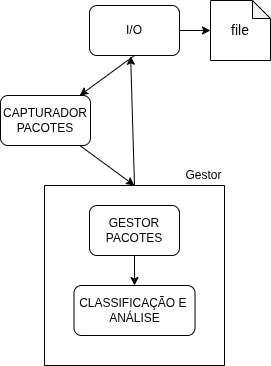
\includegraphics[width=0.40\textwidth]{images/ArquiteturaFinal.png}
        \caption{Arquitetura do sistema}
        \label{fig:arquitetura}
    \end{figure}
    \vspace{1cm}


A arquitetura do sistema desenvolvido segue uma abordagem modular, permitindo separar responsabilidades e facilitar a manutenção e evolução do sniffer de rede. O sistema é composto por vários componentes interligados que trabalham de forma sequencial desde a captura até à análise dos pacotes.

Inicialmente, o módulo de captura de pacotes é responsável por interagir diretamente com a interface de entrada/saída (I/O), recolhendo os pacotes que circulam na rede. Este componente opera em tempo real, garantindo a aquisição contínua dos dados.

De seguida, os pacotes capturados são encaminhados para o gestor de pacotes, que atua como elemento central do sistema. Este módulo é responsável por organizar o fluxo de dados, podendo realizar operações como armazenamento temporário, controlo de fluxo e preparação dos pacotes para processamento. Para além disso, o gestor coordena a comunicação entre os diferentes componentes do sistema.

Os pacotes são então enviados para o módulo de classificação e análise, onde são processados com o objetivo de identificar protocolos, extrair informação relevante e classificar o tráfego de acordo com critérios definidos.

Dependendo do modo de execução do programa, os dados são finalmente reenviados para o módulo de I/O, sendo posteriormente apresentados no terminal e/ou escritos em ficheiro. Este mecanismo permite flexibilidade na forma como os resultados são disponibilizados ao utilizador.

De forma geral, o sistema funciona como uma sequência de etapas: os pacotes são capturados, organizados, analisados e depois enviados de volta para saída. Esta organização facilita a separação de tarefas e torna o sistema mais simples de entender, manter e adaptar.

\subsection{Capturador de Pacotes}
O módulo de captura de pacotes é responsável por recolher, em tempo real, o tráfego que circula na interface de rede selecionada. Para isso, recorre à biblioteca Scapy, que permite aceder diretamente aos pacotes ao nível da rede.

A captura é iniciada com base na interface definida pelo utilizador e executada numa thread separada, permitindo que o resto do sistema (interface e processamento) continue a funcionar de forma independente:

\vspace{0.15cm}
\begin{lstlisting}
sniff(
    iface=self.iface,
    prn=handle_packet,
    store=False,
    stop_filter=lambda x: not self.running
)
\end{lstlisting}
\vspace{0.15cm}

Cada pacote capturado é imediatamente encaminhado para a função de tratamento (handle-packet), integrando-se no fluxo principal do sistema.

A utilização de uma thread dedicada garante que a captura não bloqueia a execução da aplicação:

\vspace{0.15cm}
\begin{lstlisting}
self.thread = threading.Thread(target=_sniff)
self.thread.start()
\end{lstlisting}
\vspace{0.15cm}

O módulo permite ainda controlar o ciclo de vida da captura, podendo esta ser iniciada e parada de forma controlada pelo utilizador.

De forma geral, o capturador atua como ponto de entrada do sistema, assegurando a recolha contínua e eficiente dos pacotes que serão posteriormente analisados.

\subsection{Classificação e Análise}
O módulo de classificação e análise é responsável por transformar os pacotes capturados (dados brutos) em informação estruturada e compreensível. Este processo inicia-se na função classify-packet, que cria uma estrutura base onde serão armazenados os dados extraídos:

\vspace{0.15cm}
\begin{lstlisting}
result = {
    "timestamp": datetime.now().isoformat(timespec="seconds"),
    "length":    len(raw),
    "protocol":  "OTHER",
    "summary":   "",
    "details":   {},
}
\end{lstlisting}
\vspace{0.15cm}

A análise segue uma abordagem em camadas, começando pelo nível mais baixo (Ethernet) e avançando progressivamente para níveis superiores. Cada camada é responsável por interpretar uma parte específica do pacote e decidir qual o próximo passo:

\vspace{0.15cm}
\begin{lstlisting}
parse_ethernet(raw, result)
\end{lstlisting}
\vspace{0.15cm}

Por exemplo, ao analisar um pacote IPv4, o sistema identifica o protocolo de transporte e encaminha automaticamente o processamento para o parser adequado:

\vspace{0.15cm}
\begin{lstlisting}
parser = _TRANSPORT.get(proto)
if parser:
    return parser(raw, transport_offset, result)
\end{lstlisting}
\vspace{0.15cm}

Este mecanismo permite suportar diferentes protocolos como TCP, UDP e ICMP, cada um com o seu próprio parser, responsável por extrair informação relevante como portas, flags ou tipos de mensagem. O mesmo princípio aplica-se a outros protocolos como ARP ou IPv6.
Ao longo deste processo, a informação vai sendo acumulada no campo details, enquanto é construída uma descrição resumida no campo summary, que permite uma leitura rápida do pacote (por exemplo, identificação de serviços ou tipo de comunicação).
Um aspeto relevante é a validação de alguns campos críticos, como checksums, que permite verificar a integridade dos dados analisados.
A arquitetura adotada é modular e extensível: cada protocolo está isolado no seu próprio parser, o que facilita a manutenção e permite adicionar novos protocolos com impacto mínimo no sistema. Esta abordagem tira partido da estrutura global do projeto, onde o processamento está desacoplado da captura e da visualização.
De forma geral, este módulo funciona como o núcleo do sistema, sendo responsável por converter dados binários em informação útil, que depois pode ser filtrada, apresentada ou armazenada.

\subsection{Filtragem}
O sistema inclui um mecanismo de filtragem que permite limitar os pacotes apresentados ao utilizador com base em critérios como protocolo, endereço IP ou endereço MAC. Estes filtros podem ser definidos dinamicamente durante a execução, tanto na interface TUI como GUI.

A filtragem é aplicada através de um componente dedicado, sendo os critérios armazenados internamente e utilizados sempre que um pacote é processado. De forma simplificada, o sistema verifica se cada pacote cumpre as condições definidas:

\vspace{0.15cm}
\begin{lstlisting}
if self.filter.apply(packet):
    self.output.write_packet(packet)
\end{lstlisting}
\vspace{0.15cm}

Para além da filtragem em tempo real, também é possível aplicar os mesmos critérios sobre pacotes já capturados, permitindo ao utilizador consultar apenas a informação relevante:

\vspace{0.15cm}
\begin{lstlisting}
def get_filtered_packets(self):
    return self.filter.filter_list(self.packets)
\end{lstlisting}
\vspace{0.15cm}

Desta forma, o mecanismo de filtragem atua como uma camada intermédia entre a captura e a apresentação dos dados, garantindo que apenas os pacotes de interesse são visualizados ou analisados.

\subsection{Mecanismo de Logging}
O sistema implementa um mecanismo de logging que permite guardar os pacotes capturados em ficheiro no formato JSON. Esta funcionalidade é controlada através de argumentos fornecidos na linha de comandos, permitindo ao utilizador definir o modo de execução e o ficheiro de saída.

Na fase de inicialização, são definidos os parâmetros relevantes:

\vspace{0.15cm}
\begin{lstlisting}
parser.add_argument("--mode", choices=["live", "log", "both"], required=True)
parser.add_argument("--logfile", default="logs/sniffer.json")
\end{lstlisting}
\vspace{0.15cm}

O argumento --mode permite escolher se os pacotes são apenas apresentados no terminal (live), apenas guardados em ficheiro (log), ou ambos (both). Já o argumento --logfile define o caminho do ficheiro onde os dados serão armazenados.

O processo de escrita é tratado pela classe LogOutput, responsável por gerir o ficheiro e os dados:

\vspace{0.15cm}
\begin{lstlisting}
class LogOutput:
    def __init__(self, filename):
        os.makedirs(os.path.dirname(filename), exist_ok=True)
        self.filename = filename
        self.packets = []
\end{lstlisting}
\vspace{0.15cm}

Nesta fase, é garantida a existência da diretoria onde o ficheiro será guardado, evitando erros durante a escrita.

Sempre que um pacote é capturado e processado, este é convertido para dicionário e adicionado à lista interna, sendo depois escrito no ficheiro:

\vspace{0.15cm}
\begin{lstlisting}
def write_packet(self, packet):
    self.packets.append(packet.to_dict())
    self._save()
\end{lstlisting}
\vspace{0.15cm}

A função save trata da escrita em formato JSON:

\vspace{0.15cm}
\begin{lstlisting}
def _save(self):
    with open(self.filename, "w") as f:
        json.dump(self.packets, f, indent=4)
\end{lstlisting}
\vspace{0.15cm}


Este mecanismo de logging permite ao sistema registar de forma contínua toda a informação relevante dos pacotes capturados, independentemente do modo de execução escolhido. Ao guardar os dados em formato JSON, garante-se que estes ficam organizados e fáceis de reutilizar para análise posterior. Desta forma, o logging não serve apenas como armazenamento, mas também como suporte para validação, debug e estudo do tráfego de rede capturado.

\section{Resultados}
\subsection{Topologia Core}
Foi utilizada uma topologia simples composta por dois nós ligados através de um router. O sniffer foi executado num dos nós, associado à interface de rede virtual, permitindo capturar o tráfego gerado entre os dispositivos.

A Figura \ref{fig:core1} apresenta a topologia utilizada, bem como a execução do sniffer em modo TUI durante a captura de pacotes.

\begin{figure}[H]
        \centering
        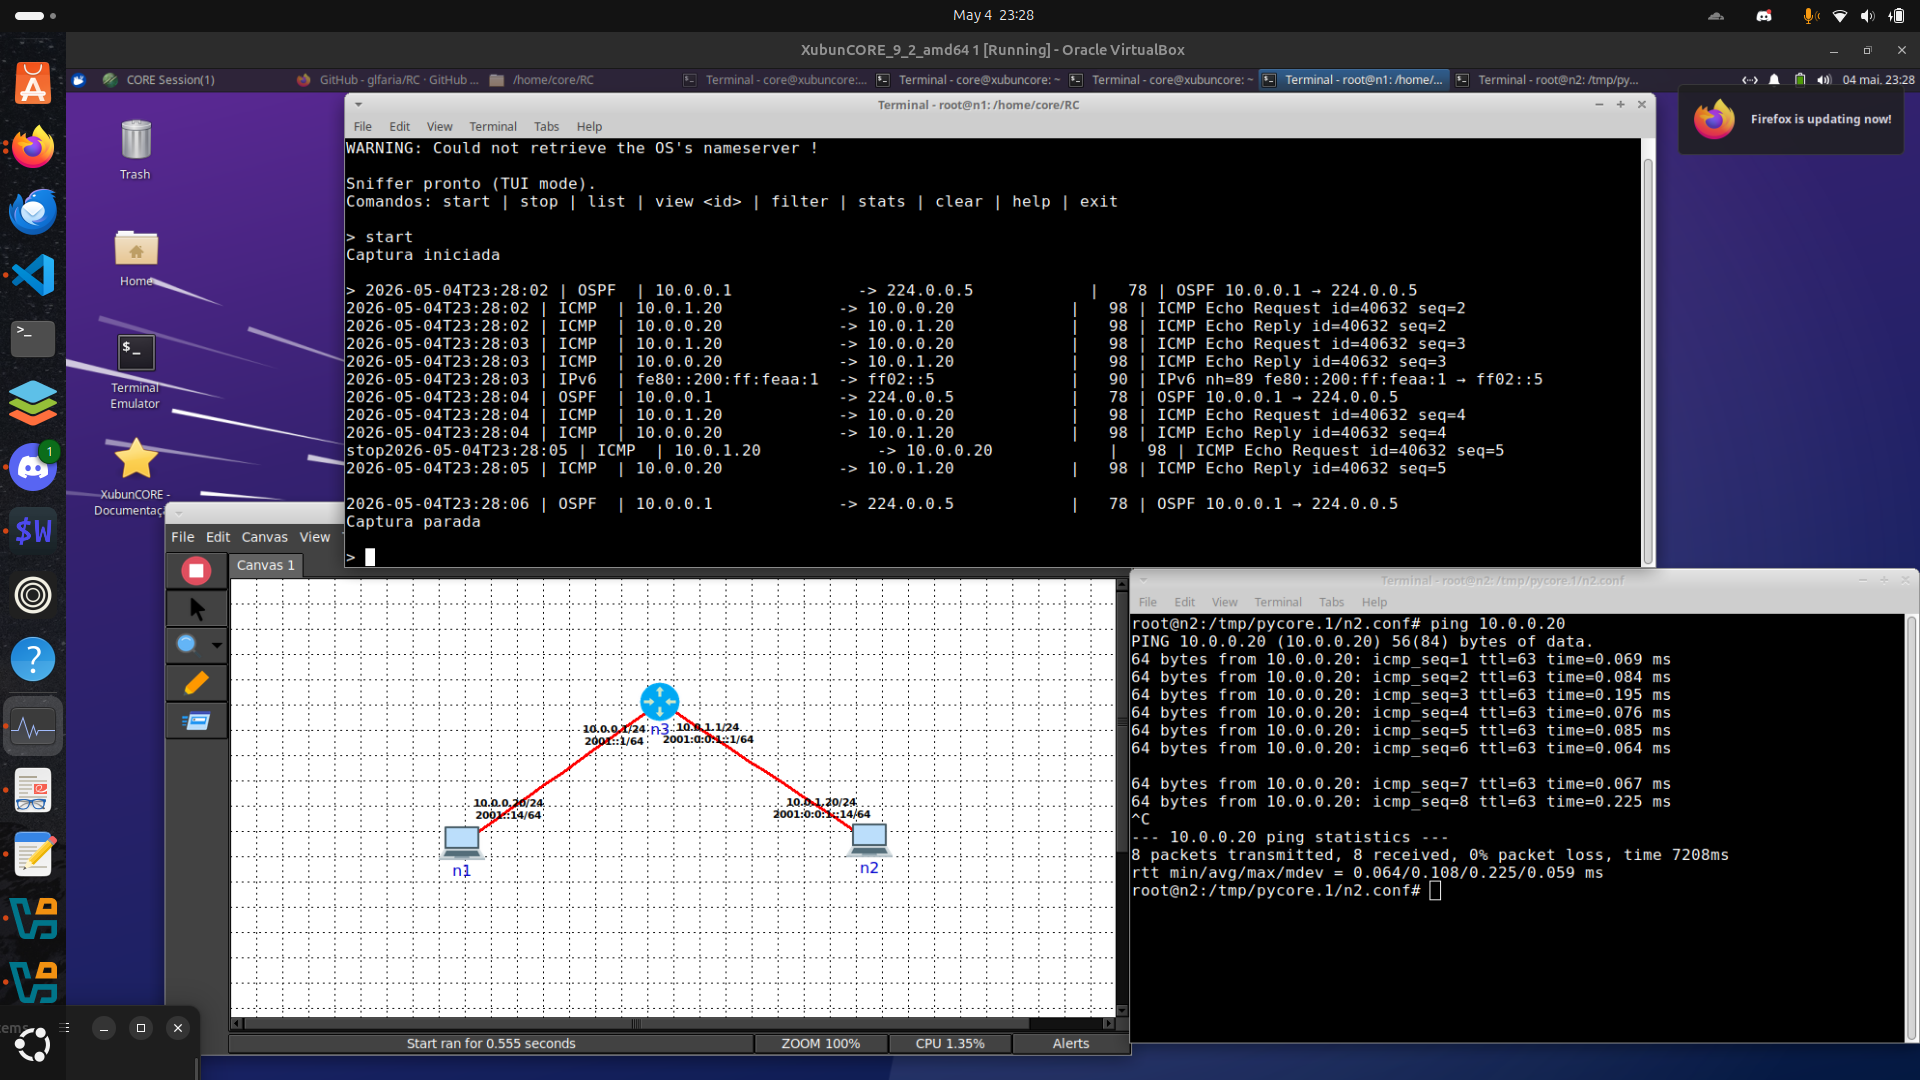
\includegraphics[width=0.9\linewidth]{images/core1.png}
        \caption{Captura de pacotes em ambiente CORE (ICMP)}
        \label{fig:core1}
    \end{figure}


Foi realizado um teste de conectividade recorrendo ao comando ping, gerando tráfego ICMP entre os nós. O sniffer capturou corretamente pacotes do tipo Echo Request e Echo Reply, sendo possível observar a correspondência entre os pedidos enviados e as respostas recebidas.

A Figura \ref{fig:core2} mostra a listagem dos pacotes capturados, evidenciando a sequência das mensagens ICMP.

\begin{figure}[H]
        \centering
        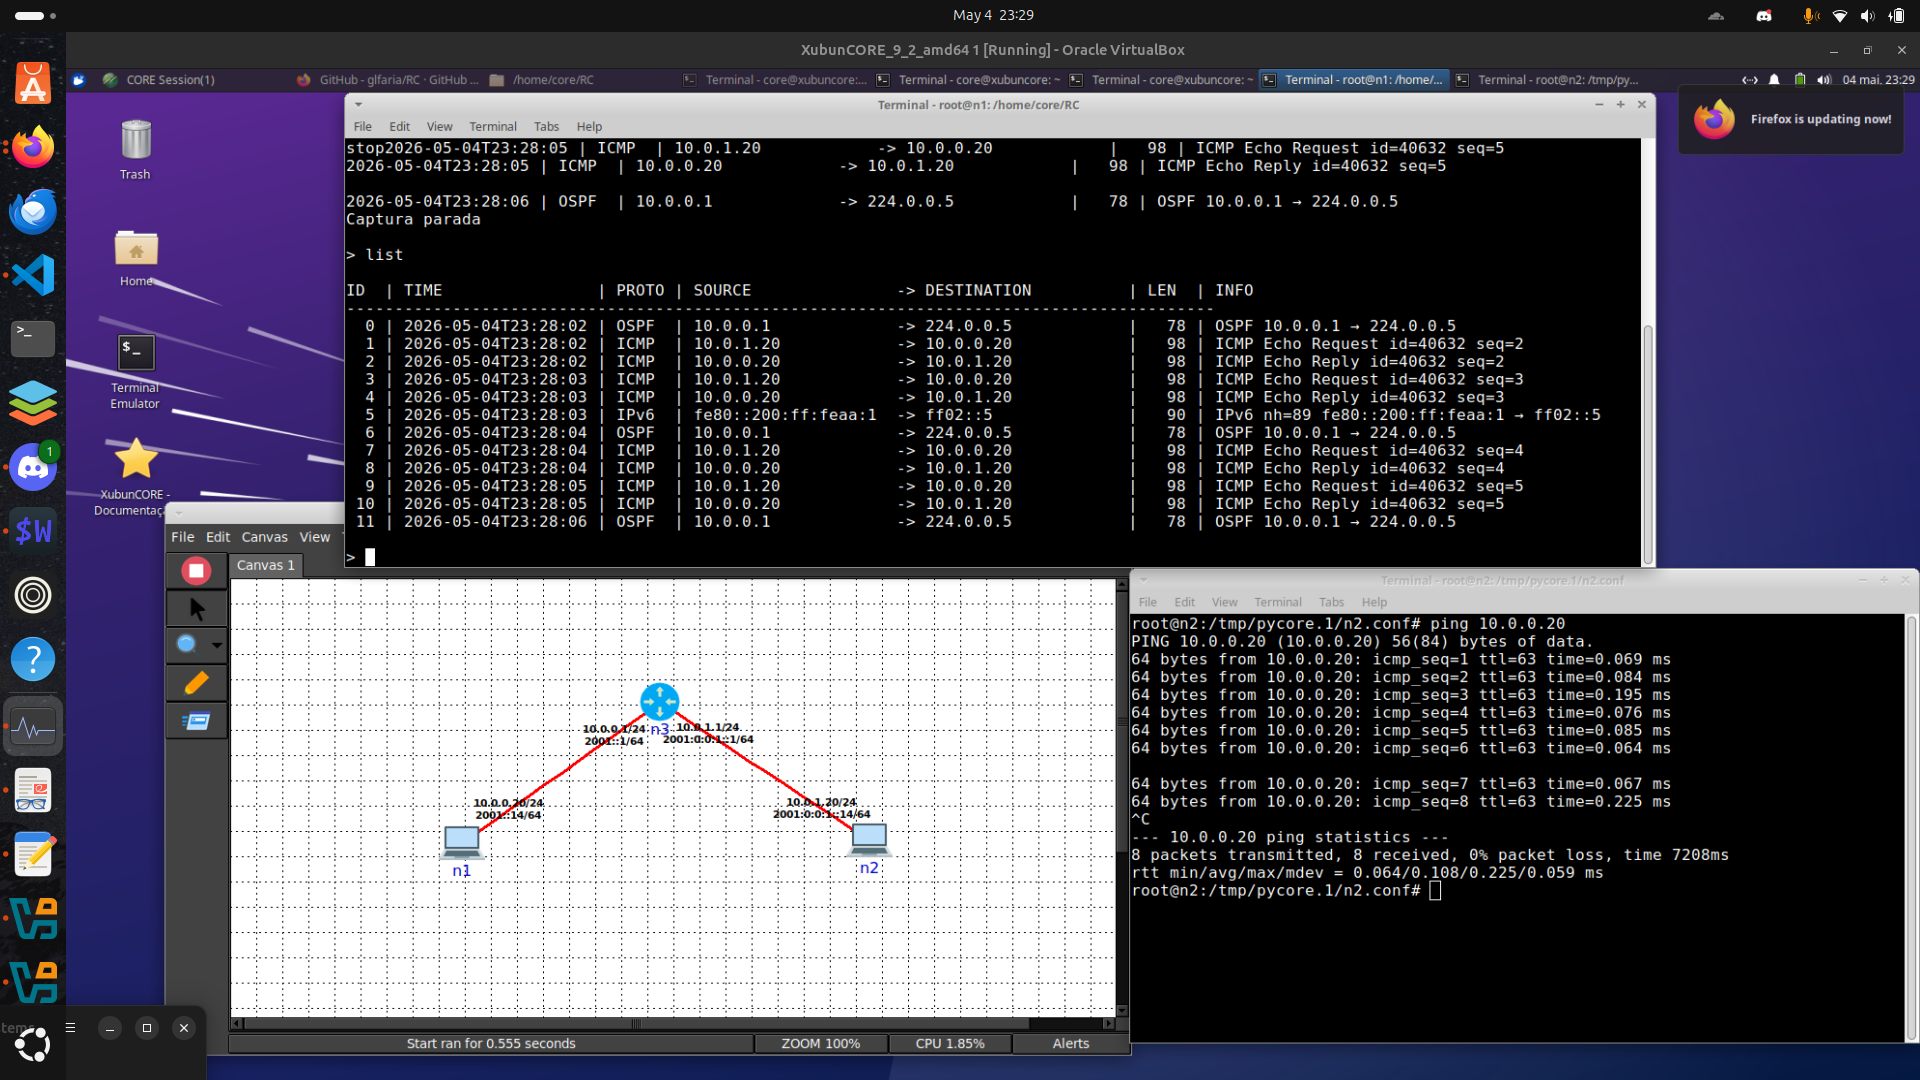
\includegraphics[width=0.9\linewidth]{images/core2.png}
        \caption{Listagem de pacotes ICMP capturados}
        \label{fig:core2}
    \end{figure}

Para validar a análise de protocolos com ligação, foi estabelecida uma comunicação TCP utilizando a ferramenta netcat. Durante este processo, o sniffer capturou o estabelecimento da ligação (three-way handshake), bem como os pacotes trocados entre cliente e servidor.

Adicionalmente, foi aplicada filtragem por endereço IP, permitindo visualizar apenas os pacotes relevantes para a comunicação em análise.

A Figura \ref{fig:core3} ilustra este cenário, mostrando os pacotes TCP capturados e filtrados.

\begin{figure}[H]
        \centering
        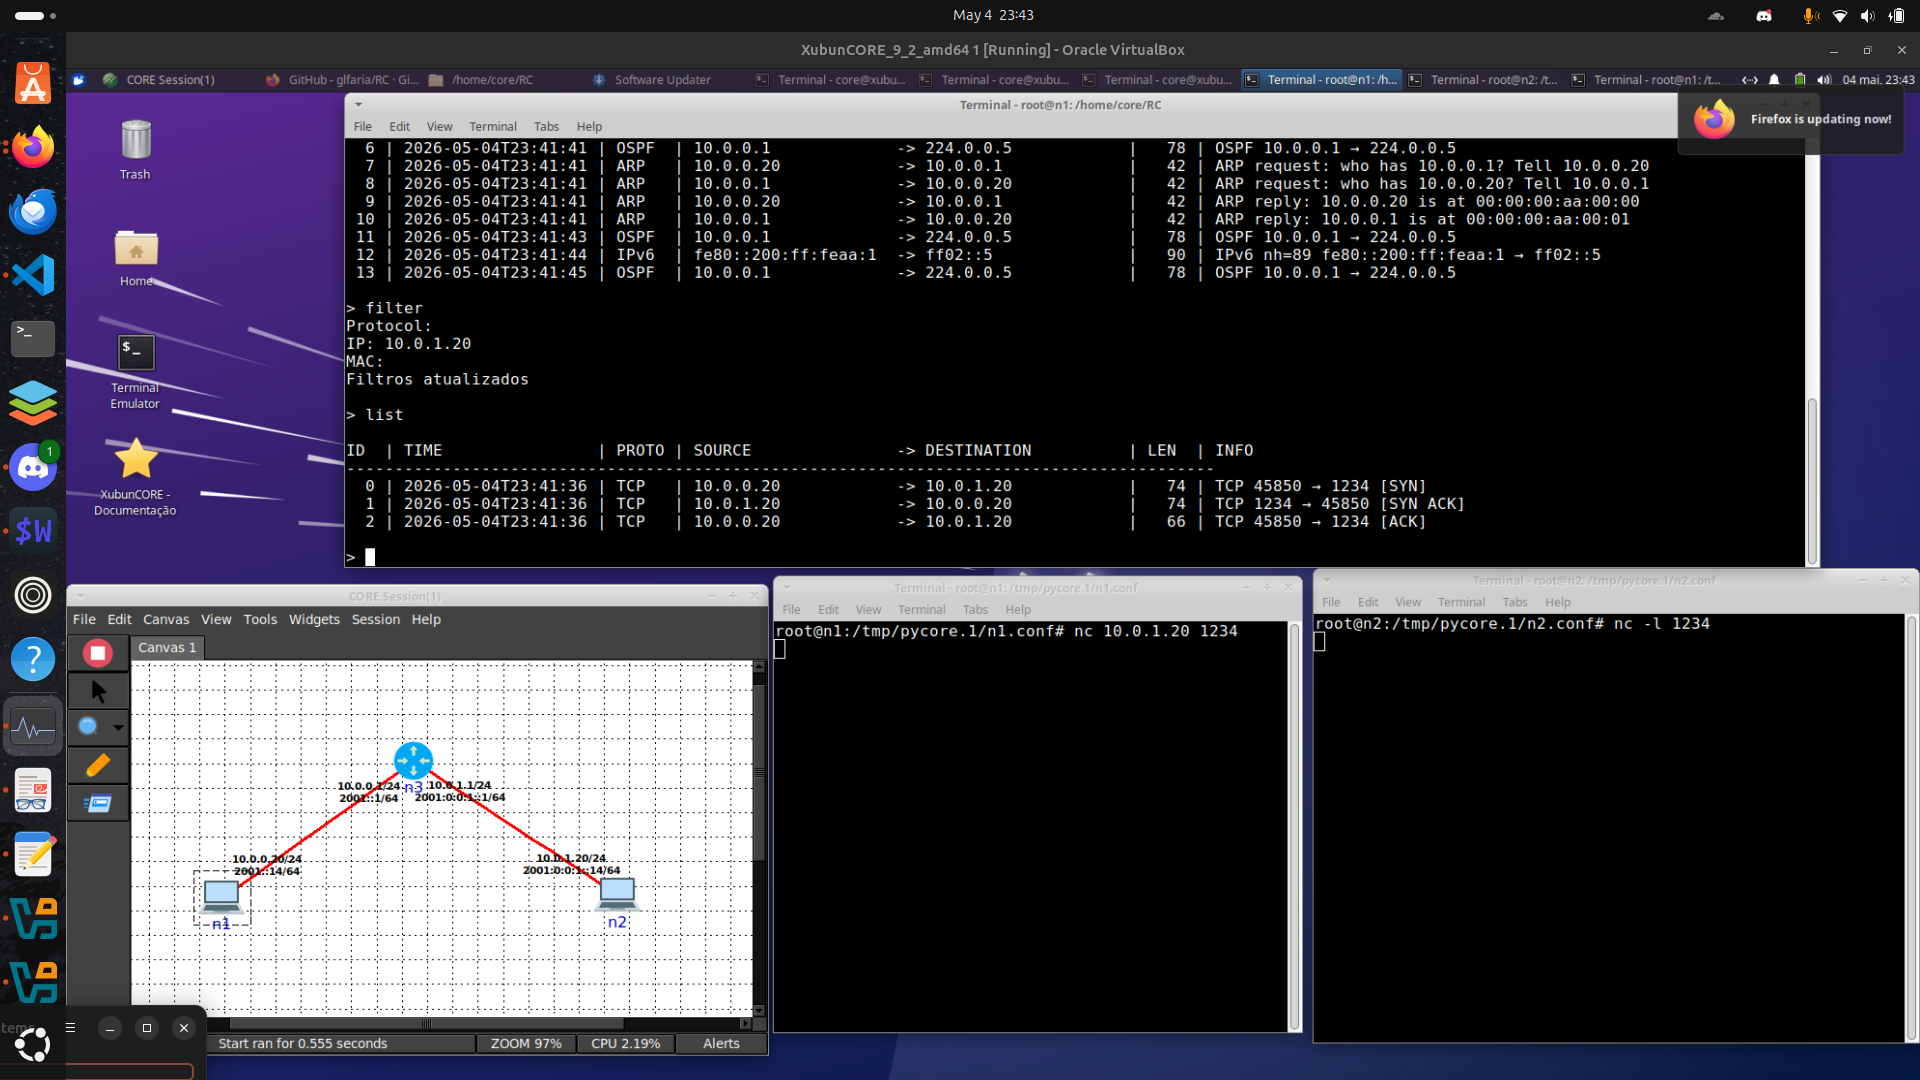
\includegraphics[width=0.9\linewidth]{images/core3.png}
        \caption{Captura e filtragem de tráfego TCP}
        \label{fig:core3}
    \end{figure}

Os testes realizados demonstram que o sistema é capaz de capturar, classificar e apresentar corretamente diferentes tipos de tráfego de rede. Foi possível validar o funcionamento tanto para protocolos sem ligação (ICMP) como para protocolos orientados à ligação (TCP), bem como a eficácia dos mecanismos de filtragem implementados.

\subsection{Validação do Funcionamento da Aplicação}
Foram realizados testes funcionais ao sniffer com o objetivo de validar a correta captura, classificação e apresentação dos pacotes de rede. Inicialmente, verificou-se o comportamento da aplicação com pacotes inválidos ou incompletos, garantindo que estes são tratados sem causar falhas. De seguida, testou-se a identificação dos principais protocolos suportados (ARP, IPv4, TCP, UDP e ICMP), confirmando que o classifier extrai corretamente os campos relevantes, como endereços IP/MAC e portas. A aplicação foi ainda executada em modo “live” e “log”, validando tanto a impressão em tempo real como o registo em ficheiro. Foram também utilizados os filtros disponíveis (por protocolo, IP e MAC), verificando-se que estes limitam corretamente os pacotes apresentados. Por fim, a execução numa interface real permitiu observar tráfego legítimo (nomeadamente TCP e UDP), comprovando o funcionamento global do sistema em ambiente real.

\section{Conclusão}
O desenvolvimento deste sniffer permitiu consolidar a compreensão prática da estrutura hierárquica dos protocolos de rede e do modo como estes se relacionam na transmissão de pacotes. A aplicação desenvolvida foi capaz de capturar e interpretar tráfego em ambiente controlado no CORE e numa interface real do computador, identificando corretamente protocolos como ARP, IPv4, ICMP, TCP e UDP, bem como os campos mais relevantes dos respetivos cabeçalhos. Na interface real, foi possível observar tráfego mais variado e dinâmico do que no emulador, incluindo comunicações TCP/UDP associadas a serviços externos, o que reforçou a utilidade do sniffer para análise de tráfego real. 

Apesar dos resultados obtidos, a aplicação apresenta algumas limitações. A mais relevante prende-se com o facto de não ter sido implementada a associação explícita entre as capturas observadas e diagramas de funcionamento dos protocolos, conforme indicado nos requisitos do enunciado. Além disso, a análise foi concentrada sobretudo nas camadas de ligação, rede e transporte, não tendo sido feita uma reconstrução completa de fluxos nem uma dissecação profunda da camada de aplicação. Também não foram implementadas funcionalidades mais avançadas, como reassemblagem de segmentos, suporte extensivo a protocolos adicionais ou visualizações gráficas mais elaboradas. Ainda assim, o trabalho desenvolvido cumpre os objetivos principais definidos, fornecendo uma base funcional, modular e extensível para captura, classificação, filtragem e registo de tráfego.

Em síntese, este projeto permitiu desenvolver uma ferramenta funcional de análise passiva de pacotes, com uma arquitetura organizada e facilmente expansível, e com capacidade para ser utilizada tanto em ambiente emulado como em rede real. O trabalho realizado evidenciou a importância do parsing manual dos cabeçalhos para compreender o funcionamento dos protocolos e confirmou a utilidade de um sniffer próprio para apoiar a análise e o estudo das comunicações em rede.

\end{document}